\documentclass[tikz,border=10pt]{standalone}
\usepackage{tkz-euclide} % 增强几何绘图宏包
\begin{document}
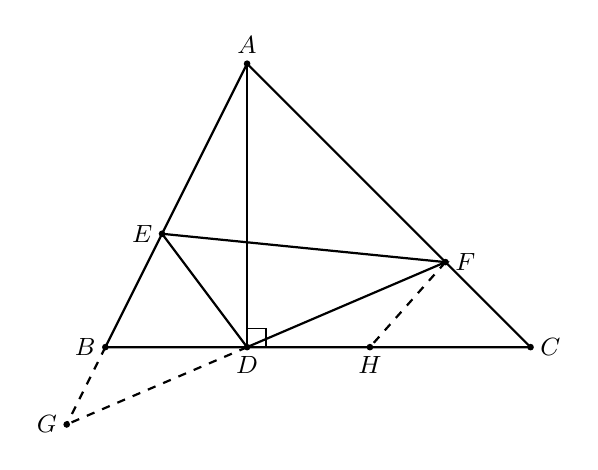
\begin{tikzpicture}[scale=1.2, font=\small]    
% 1. 定义基本顶点坐标 (基于图像比例估算)    
\coordinate (A) at (1.5, 4);    
\coordinate (B) at (0, 1);    
\coordinate (C) at (4.5, 1);        
% 2. 计算点 D (A到BC的垂足)    
\coordinate (D) at (1.5, 1);        
% 3. 定义点 E 和 F (分别在 AB 和 AC 边上)    
\coordinate (E) at ($(A)!0.6!(B)$); % E在AB上靠近B的位置    
\coordinate (F) at ($(A)!0.7!(C)$); % F在AC上靠近C的位置        
% 4. 计算辅助点 G (直线 AB 与 DF 的交点)    
\coordinate (G) at (intersection of A--B and D--F);        
% 5. 定义 H 点 (在 BC 上)    
\coordinate (H) at (2.8, 1);
    % --- 绘制线条 ---        
% 实线部分：大三角形与内部连接线    
\draw[thick] (A) -- (B) -- (C) -- cycle;    
\draw[thick] (A) -- (D);    
\draw[thick] (E) -- (D) -- (F) -- cycle;        
% 虚线部分：延长线与辅助线    
\draw[dashed, thick] (B) -- (G);   % AB的延长线    
\draw[dashed, thick] (D) -- (G);   % DF的延长线    
\draw[dashed, thick] (F) -- (H);   % FH 辅助线
    % 6. 标注直角符号 (AD 垂直 BC)    
\draw (1.5, 1.2) -- (1.7, 1.2) -- (1.7, 1);
    % --- 标注字母 ---    
% 按方位放置标签以避免重叠    
\node[above] at (A) {$A$};    
\node[left]  at (B) {$B$};    
\node[right] at (C) {$C$};    
\node[below] at (D) {$D$};    
\node[left]  at (E) {$E$};    
\node[right] at (F) {$F$};    
\node[left]  at (G) {$G$};    
\node[below] at (H) {$H$};
    % 绘制关键点圆点 (可选)    
\foreach \p in {A,B,C,D,E,F,G,H}        
\fill (\p) circle (1pt);
\end{tikzpicture}
\end{document}